\hypertarget{VisualBlock_8h}{
\section{/PIWO/Program/gui/VisualBlock.h File Reference}
\label{VisualBlock_8h}\index{/PIWO/Program/gui/VisualBlock.h@{/PIWO/Program/gui/VisualBlock.h}}
}
{\tt \#include $<$SysUtils.hpp$>$}\par
{\tt \#include $<$Classes.hpp$>$}\par
{\tt \#include $<$Controls.hpp$>$}\par
{\tt \#include $<$ExtCtrls.hpp$>$}\par
{\tt \#include $<$Buttons.hpp$>$}\par
{\tt \#include \char`\"{}../engine/BlockInput.h\char`\"{}}\par
{\tt \#include \char`\"{}../engine/BlockOutput.h\char`\"{}}\par
{\tt \#include \char`\"{}../engine/Block.h\char`\"{}}\par
{\tt \#include \char`\"{}VisualInput.h\char`\"{}}\par
{\tt \#include \char`\"{}VisualOutput.h\char`\"{}}\par
{\tt \#include \char`\"{}BlockHistory.h\char`\"{}}\par


Include dependency graph for VisualBlock.h:\nopagebreak
\begin{figure}[H]
\begin{center}
\leavevmode
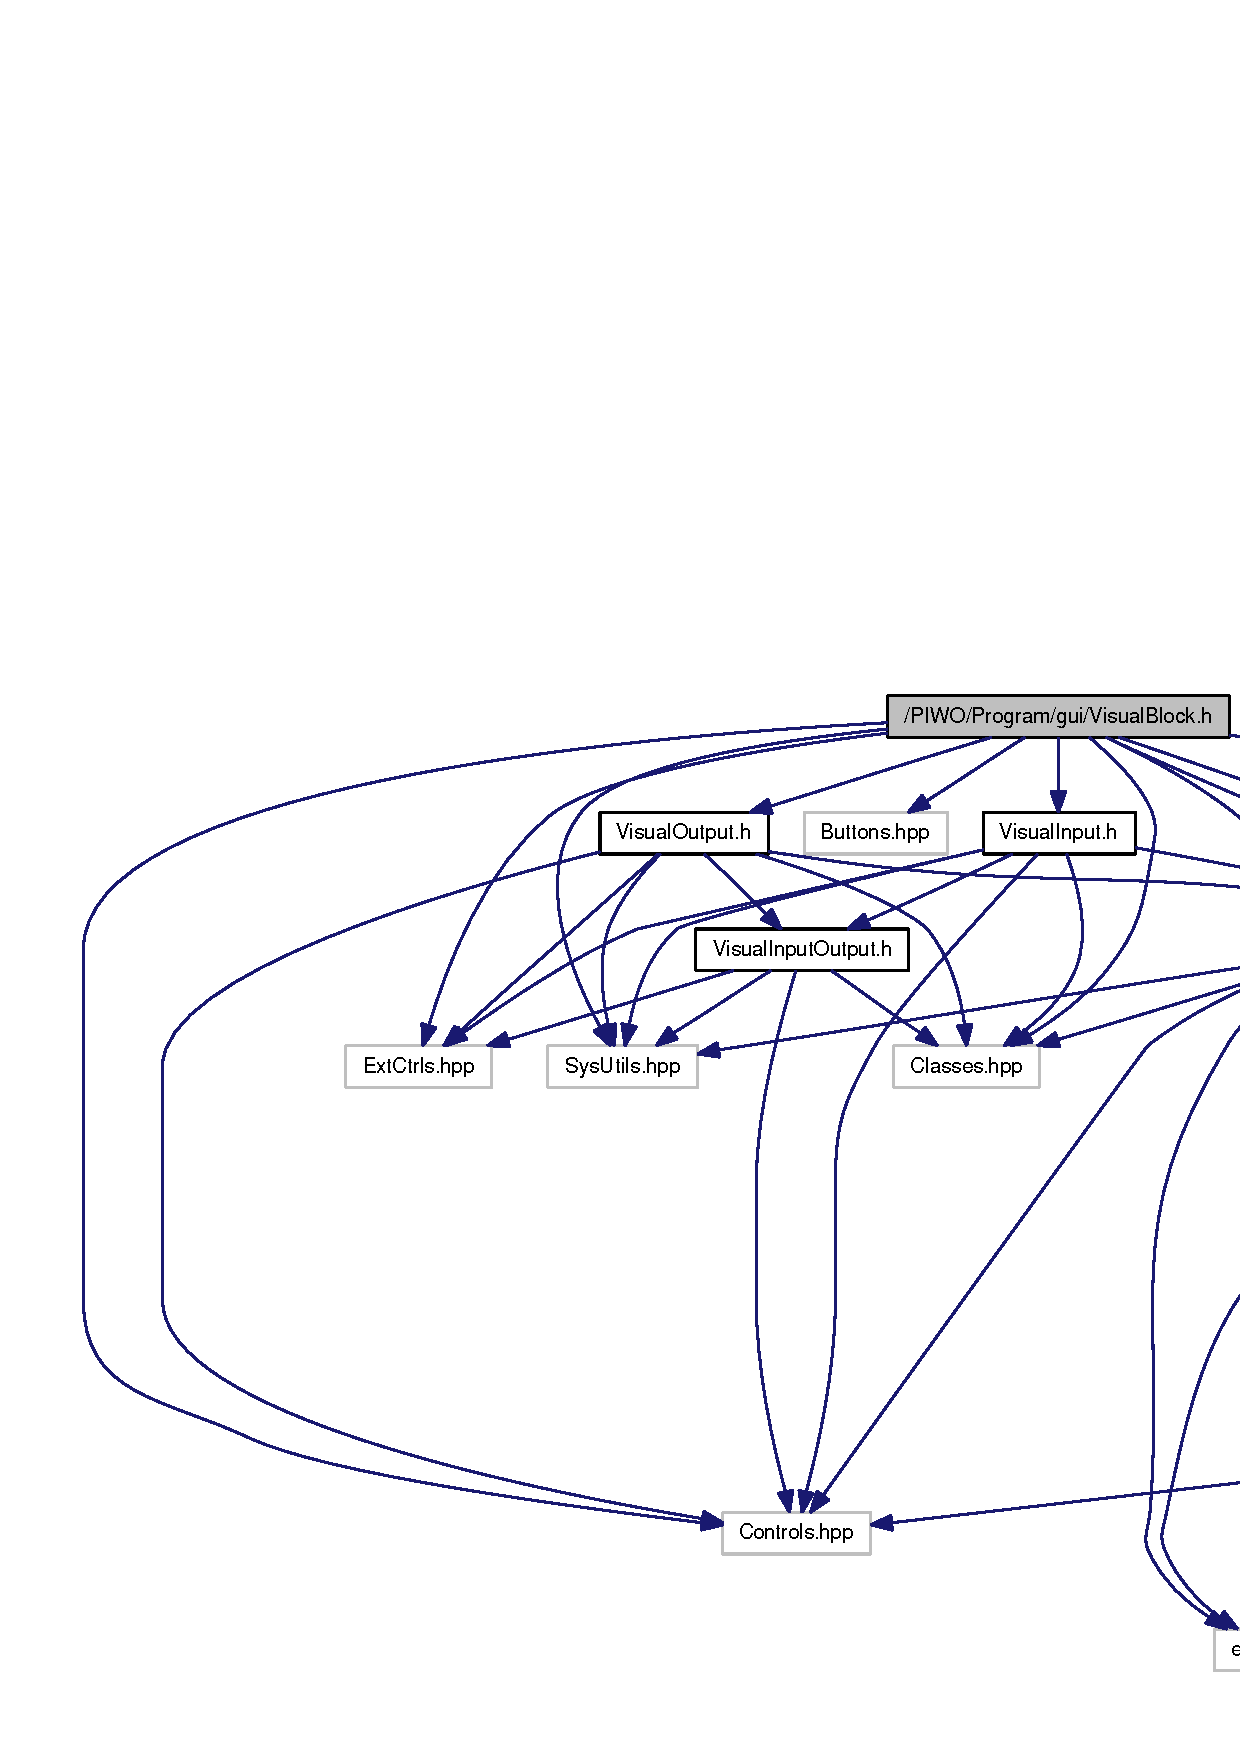
\includegraphics[width=420pt]{VisualBlock_8h__incl}
\end{center}
\end{figure}


This graph shows which files directly or indirectly include this file:\nopagebreak
\begin{figure}[H]
\begin{center}
\leavevmode
\includegraphics[width=420pt]{VisualBlock_8h__dep__incl}
\end{center}
\end{figure}
\subsection*{Classes}
\begin{CompactItemize}
\item 
struct \hyperlink{structPosition}{Position}
\item 
class \hyperlink{classVisualBlock}{VisualBlock}
\end{CompactItemize}
\subsection*{Defines}
\begin{CompactItemize}
\item 
\#define \hyperlink{VisualBlock_8h_318dcd0c0a579276e1ad2effdbd5a003}{PIWOMAINCLASSTYPE}~TScrollBox
\end{CompactItemize}
\subsection*{Typedefs}
\begin{CompactItemize}
\item 
typedef TObject $\ast$typedef TObject $\ast$typedef TObject $\ast$typedef TObject $\ast$typedef \hyperlink{VisualBlock_8h_90fab0ddf29ee9641b22d2f86d8e7896}{bool}
\item 
typedef TObject $\ast$typedef TObject $\ast$typedef TObject $\ast$typedef TObject $\ast$typedef \hyperlink{VisualBlock_8h_f335b7e3ffabe79bf5a4fa5e032998ec}{int}
\end{CompactItemize}
\subsection*{Functions}
\begin{CompactItemize}
\item 
typedef \hyperlink{VisualBlock_8h_aab8db8870823111411bee30174e8711}{void} (\_\-\_\-closure $\ast$VisualBlock\_\-FunctionI)(\hyperlink{classVisualInput}{VisualInput} $\ast$
\item 
bool \hyperlink{VisualBlock_8h_e98017465acd6b8492e2b1e0388f6baf}{ctrlDown} ()
\item 
bool \hyperlink{VisualBlock_8h_bbd7b95458674f02427af4cae5198a4e}{altDown} ()
\end{CompactItemize}


\subsection{Define Documentation}
\hypertarget{VisualBlock_8h_318dcd0c0a579276e1ad2effdbd5a003}{
\index{VisualBlock.h@{VisualBlock.h}!PIWOMAINCLASSTYPE@{PIWOMAINCLASSTYPE}}
\index{PIWOMAINCLASSTYPE@{PIWOMAINCLASSTYPE}!VisualBlock.h@{VisualBlock.h}}
\subsubsection[PIWOMAINCLASSTYPE]{\setlength{\rightskip}{0pt plus 5cm}\#define PIWOMAINCLASSTYPE~TScrollBox}}
\label{VisualBlock_8h_318dcd0c0a579276e1ad2effdbd5a003}




Definition at line 15 of file VisualBlock.h.

\subsection{Typedef Documentation}
\hypertarget{VisualBlock_8h_90fab0ddf29ee9641b22d2f86d8e7896}{
\index{VisualBlock.h@{VisualBlock.h}!bool@{bool}}
\index{bool@{bool}!VisualBlock.h@{VisualBlock.h}}
\subsubsection[bool]{\setlength{\rightskip}{0pt plus 5cm}typedef TObject$\ast$ typedef TObject$\ast$ typedef TObject$\ast$ typedef TObject$\ast$ typedef bool}}
\label{VisualBlock_8h_90fab0ddf29ee9641b22d2f86d8e7896}




Definition at line 26 of file VisualBlock.h.\hypertarget{VisualBlock_8h_f335b7e3ffabe79bf5a4fa5e032998ec}{
\index{VisualBlock.h@{VisualBlock.h}!int@{int}}
\index{int@{int}!VisualBlock.h@{VisualBlock.h}}
\subsubsection[int]{\setlength{\rightskip}{0pt plus 5cm}typedef TObject$\ast$ typedef TObject$\ast$ typedef TObject$\ast$ typedef TObject$\ast$ typedef int}}
\label{VisualBlock_8h_f335b7e3ffabe79bf5a4fa5e032998ec}




Definition at line 26 of file VisualBlock.h.

\subsection{Function Documentation}
\hypertarget{VisualBlock_8h_bbd7b95458674f02427af4cae5198a4e}{
\index{VisualBlock.h@{VisualBlock.h}!altDown@{altDown}}
\index{altDown@{altDown}!VisualBlock.h@{VisualBlock.h}}
\subsubsection[altDown]{\setlength{\rightskip}{0pt plus 5cm}bool altDown ()}}
\label{VisualBlock_8h_bbd7b95458674f02427af4cae5198a4e}


Informuje czy klawisz Alt jest wcisniety \begin{Desc}
\item[Returns:]true -wcisniety, false - nie wcisniety \end{Desc}


Definition at line 651 of file VisualBlock.cpp.

Referenced by VisualBlock::BlockClick().\hypertarget{VisualBlock_8h_e98017465acd6b8492e2b1e0388f6baf}{
\index{VisualBlock.h@{VisualBlock.h}!ctrlDown@{ctrlDown}}
\index{ctrlDown@{ctrlDown}!VisualBlock.h@{VisualBlock.h}}
\subsubsection[ctrlDown]{\setlength{\rightskip}{0pt plus 5cm}bool ctrlDown ()}}
\label{VisualBlock_8h_e98017465acd6b8492e2b1e0388f6baf}


Informuje czy klawisz Ctrl jest wcisniety \begin{Desc}
\item[Returns:]true -wcisniety, false - nie wcisniety \end{Desc}


Definition at line 644 of file VisualBlock.cpp.

Referenced by VisualBlock::BlockClick().\hypertarget{VisualBlock_8h_aab8db8870823111411bee30174e8711}{
\index{VisualBlock.h@{VisualBlock.h}!void@{void}}
\index{void@{void}!VisualBlock.h@{VisualBlock.h}}
\subsubsection[void]{\setlength{\rightskip}{0pt plus 5cm}typedef void (\_\-\_\-closure $\ast$ {\em VisualBlock\_\-FunctionI})}}
\label{VisualBlock_8h_aab8db8870823111411bee30174e8711}


